% !TeX root = ../main.tex
% !TeX encoding = UTF-8
% !TeX spellcheck = none
\section{Experiments and Analysis}\label{sec:experiments}

\subsection{Experimental Settings}\label{sec:exp-settings}

\subsubsection{Datasets, Preprocessing, and Forecasting Protocol}\label{sec:exp-datasets}

We evaluated regional traffic flow forecasting on two datasets: Chengdu DiDi ride-hailing orders collected in November 2016 and Shanghai taxi origin--destination (OD) records collected in August 2016. For each city, we selected a fixed core area and divided it into a \(32\times32\) grid. Inflow and outflow are counts per 5 min, aggregated independently from trip destinations and origins, respectively. Table~\ref{tab:dataset-summary} summarizes the datasets, and Figures~\ref{fig:chengdu-t5-dataset} and~\ref{fig:shanghai-t5-dataset} show their endpoint distributions, grid partitions, and mean flows.

Both datasets used the same cleaning and aggregation procedure, with timestamps converted to Beijing time (UTC+8). We removed exact duplicates and records with invalid timestamps or coordinates. Retained orders lasted 2--120 minutes, had both endpoints within the city's coarse geographic boundary, and had an average speed no greater than \(120\,\mathrm{km/h}\), computed from great-circle distance and trip duration. Valid endpoints in the core area were aggregated into grid cells and time intervals; cells with no endpoint events were assigned zero. Shanghai source quality was flagged as invalid from 2016-08-11 to 2016-08-14. We retained these records in the flow series and in the training-input statistics, while applying the quality mask when computing source-quality summaries and scenario references.

\begin{table}[!htbp]
	\centering
	\caption{Dataset properties and sample splits}
	\label{tab:dataset-summary}
	\small
	\begin{tabular}{lcc}
		\toprule
		Property & Chengdu & Shanghai \\
		\midrule
		Observation period & 2016-11-01 to 2016-11-30 & 2016-08-01 to 2016-08-31 \\
		Grid size & \(32\times32\) & \(32\times32\) \\
		Approx. cell dimensions (km) & \(0.42\times0.44\) & \(0.80\times0.68\) \\
		Sampling interval & 5 minutes & 5 minutes \\
		Complete time intervals & 8,640 & 8,928 \\
		Orders after cleaning & 6,082,753 & 7,744,423 \\
		Training windows & 5,170 & 5,343 \\
		Validation windows & 1,724 & 1,781 \\
		Test windows & 1,723 & 1,781 \\
		\bottomrule
	\end{tabular}
\end{table}

For each dataset, we generated stride-1 rolling-origin windows. Each window uses the past 12 observations to predict inflow and outflow over the next 12 steps, covering 60 minutes of history and forecasts. We retained the associated time-of-day and day-of-week features and kept only windows with complete inputs and targets. The resulting windows were ordered by forecast origin and divided chronologically into training, validation, and test sets at an approximate ratio of 6:2:2 (Table~\ref{tab:dataset-summary}). This rolling-origin protocol preserves temporal order while allowing each forecast origin to use the immediately preceding observations as history. All methods used the same ordered indices and forecasting task.

For each flow channel, standardization means and standard deviations were computed from the historical inputs of training windows and fixed for validation and testing. Predictions were returned to the original flow scale by channel-wise inverse standardization. Section~\ref{sec:exp-implementation} describes checkpoint selection, and Section~\ref{sec:exp-baselines-metrics} defines the evaluation metrics.

\begin{figure}[!htbp]
	\centering
	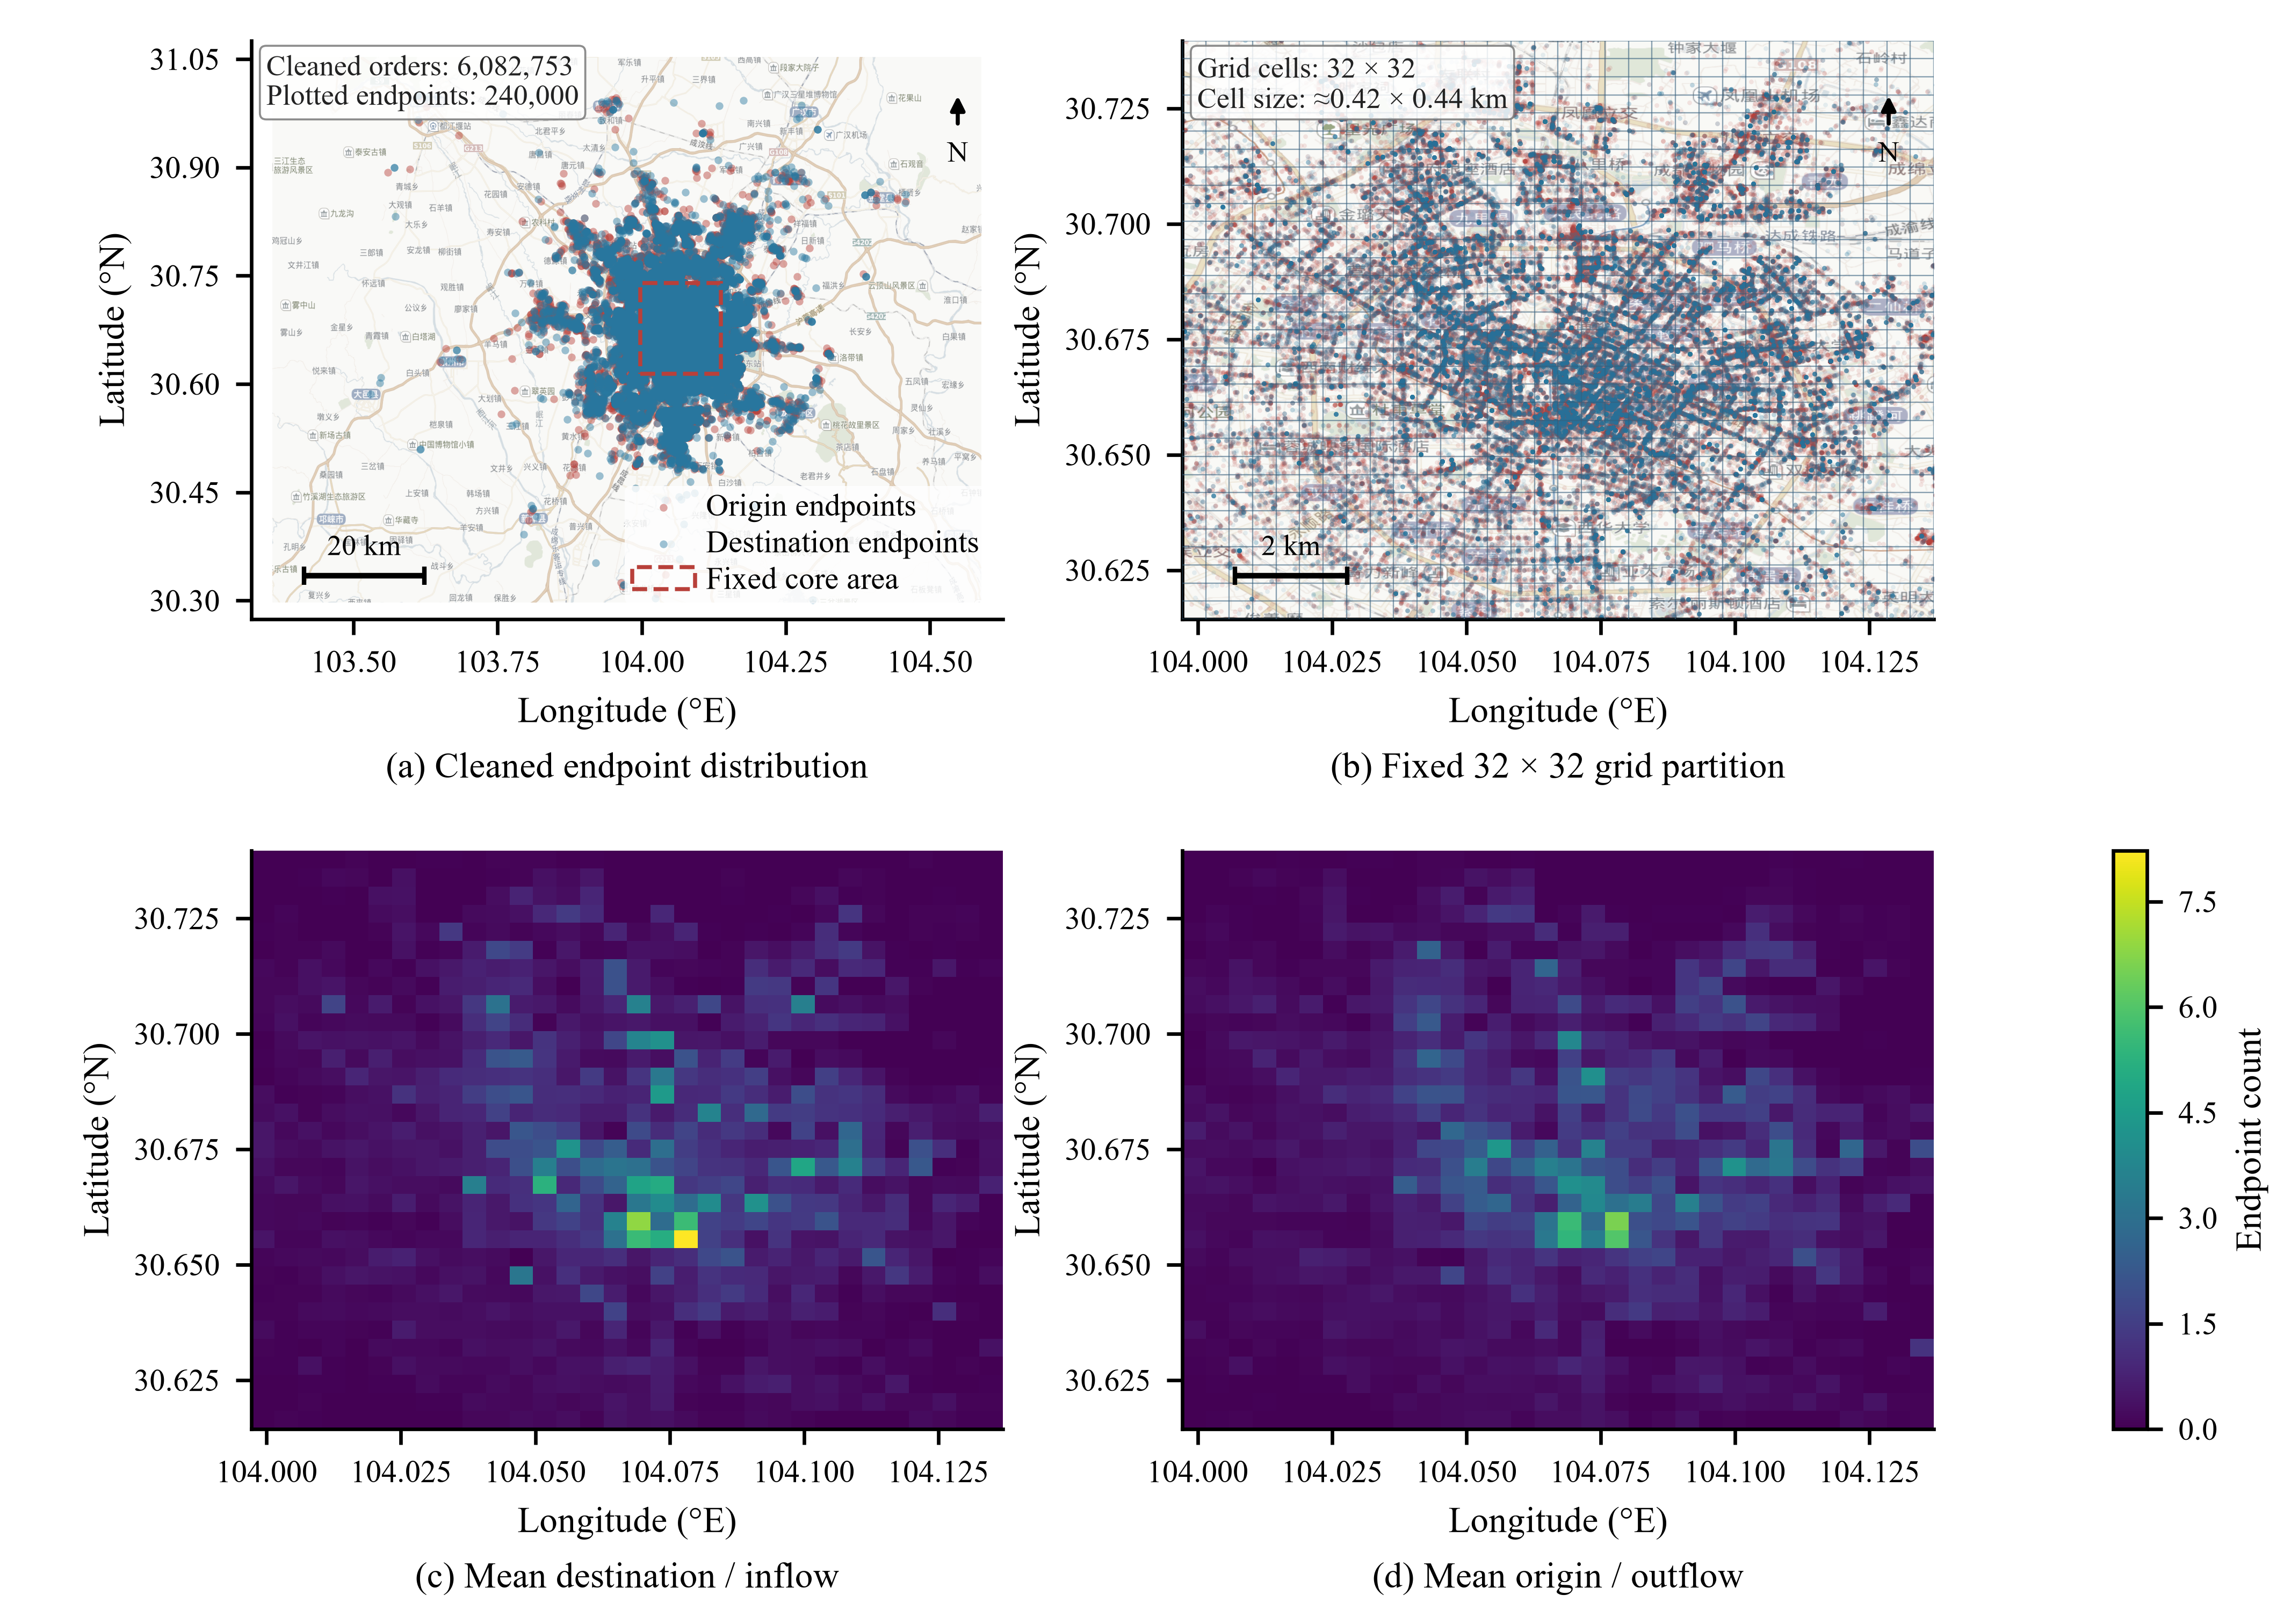
\includegraphics[width=\linewidth]{figures/chengdu-t5-overview.png}
\caption{Chengdu endpoint distribution, grid partition, and mean flow.}
	\label{fig:chengdu-t5-dataset}
\end{figure}

\begin{figure}[!htbp]
	\centering
	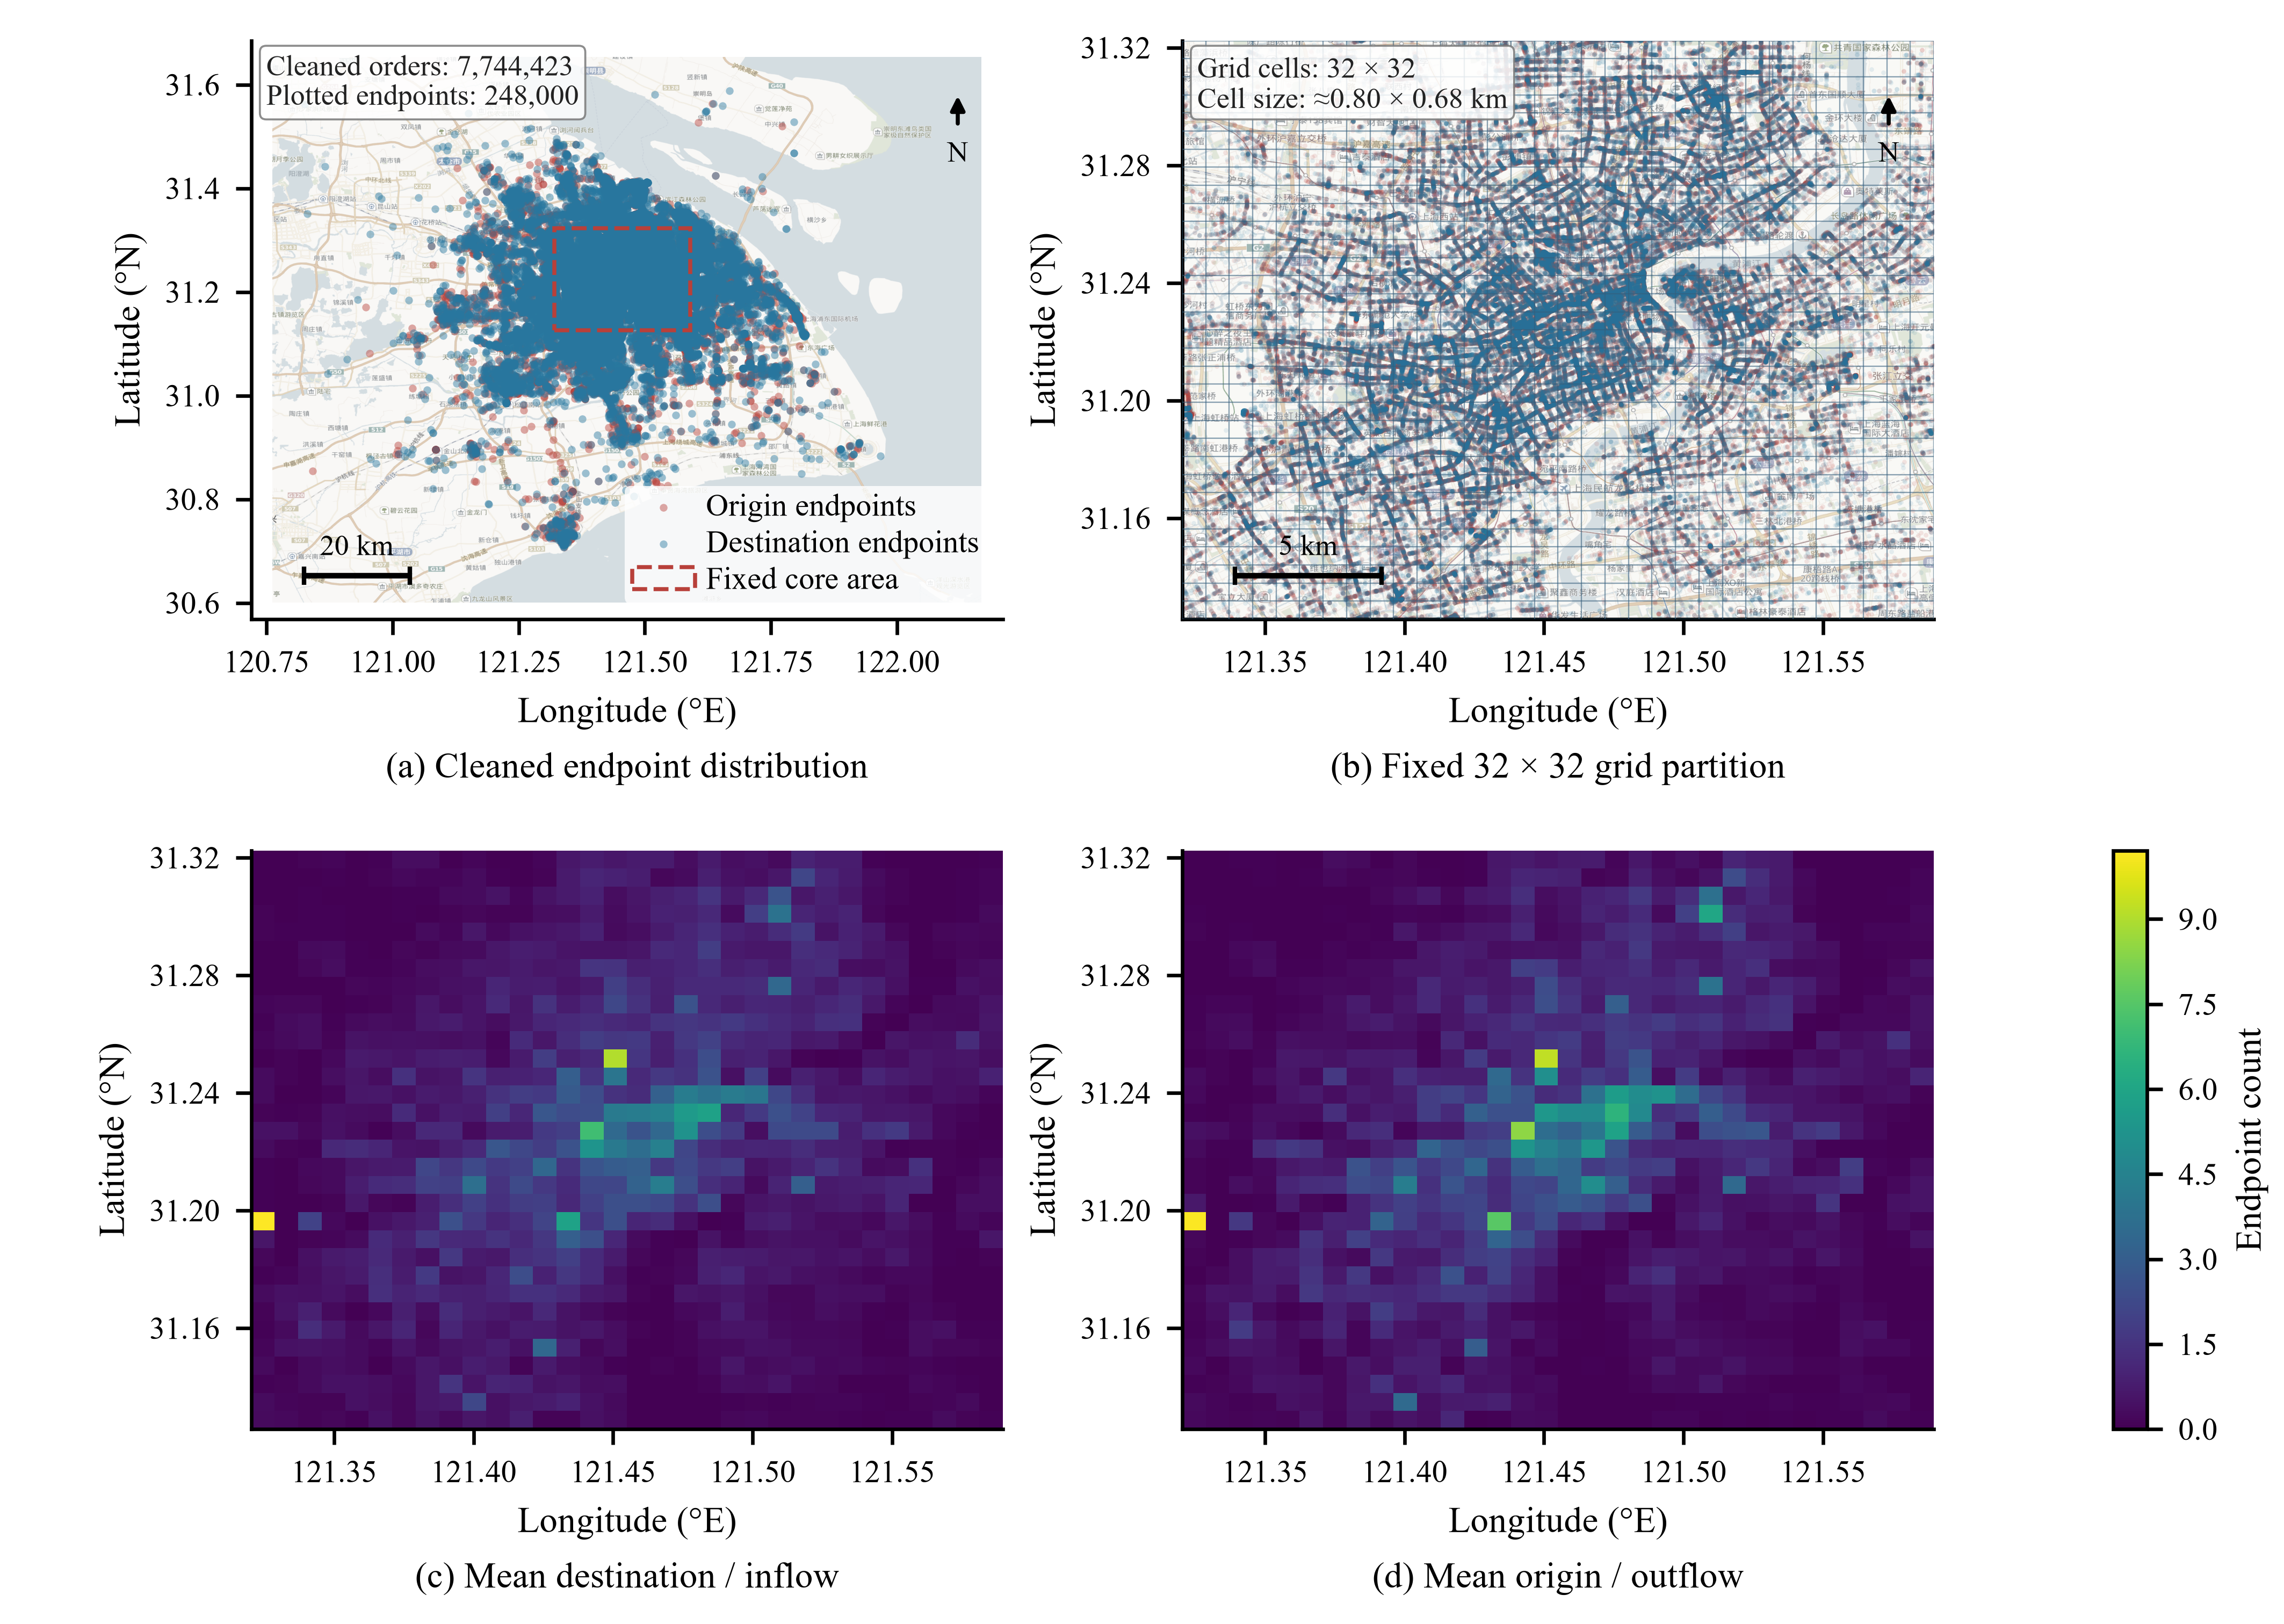
\includegraphics[width=\linewidth]{figures/shanghai-t5-overview.png}
\caption{Shanghai endpoint distribution, grid partition, and mean flow.}
	\label{fig:shanghai-t5-dataset}
\end{figure}

\subsubsection{Baseline Methods and Evaluation Metrics}\label{sec:exp-baselines-metrics}

The main experiments compared RBSRN with 13 baselines from three forecasting paradigms. Conventional methods were historical average (HA) and support vector regression (SVR). Deep models were DCRNN~\cite{ref01}, STGCN~\cite{ref02}, Graph WaveNet (GWNet)~\cite{ref03}, DSTAGNN~\cite{ref19}, PDFormer~\cite{ref10}, STDN~\cite{ref20}, MetaDG~\cite{ref21}, HyperD~\cite{ref22}, and RAST~\cite{ref23}; general time-series models were PatchTST~\cite{ref12} and TimeMixer~\cite{ref13}. Every method used the chronological split and 12-step task defined above. Inflow and outflow were evaluated separately in each city.

The scenario analysis additionally included vector autoregression (VAR), STNorm~\cite{ref24}, and STWave~\cite{ref11}, for 16 baselines in total.

We use mean absolute error (MAE) and root mean squared error (RMSE), computed on the original flow scale after inverse standardization. The main tables use a positive-target mask and evaluate locations with observed flow greater than zero. The scope-sensitivity analysis applies the same RBSRN checkpoint to all grid cells, including zero targets; it characterizes metric sensitivity rather than reranking baselines. Let \(\mathcal{T}_{\mathrm{test}}\) denote the forecast origins of the actual test windows. Let \(y_{t,h,i,c}\) and \(\widehat y_{t,h,i,c}\) denote the observed and predicted values for forecast origin \(t\), forecast step \(h\), grid cell \(i\), and channel \(c\in\{\mathrm{in},\mathrm{out}\}\). The prediction error is \(e_{t,h,i,c}=\widehat y_{t,h,i,c}-y_{t,h,i,c}\). The two evaluation scopes are
\[
\begin{aligned}
	\Omega^{+}_{h,c}&=\bigl\{(t,i)\mid t\in\mathcal{T}_{\mathrm{test}},\ 1\leq i\leq N,\ y_{t,h,i,c}>0\bigr\},\\
	\Omega^{\mathrm{all}}_{h,c}&=\mathcal{T}_{\mathrm{test}}\times\{1,\ldots,N\}.
\end{aligned}
\]
For \(m\in\{+,\mathrm{all}\}\), we pool all test windows and nodes within the corresponding scope to compute
\begin{equation}
	\label{eq:eval-mae}
	\mathrm{MAE}^{m}_{h,c}
	=\frac{1}{|\Omega^{m}_{h,c}|}
	\sum_{(t,i)\in\Omega^{m}_{h,c}}|e_{t,h,i,c}|,
\end{equation}
\begin{equation}
	\label{eq:eval-rmse}
	\mathrm{RMSE}^{m}_{h,c}
	=\sqrt{\frac{1}{|\Omega^{m}_{h,c}|}
		\sum_{(t,i)\in\Omega^{m}_{h,c}}e_{t,h,i,c}^{2}}.
\end{equation}
Here, \(|\Omega^{m}_{h,c}|\) is the number of evaluated locations. Both scopes exclude duplicate windows introduced by test-batch padding, and inflow and outflow are evaluated separately.

We report the single-step results H3, H6, and H12, corresponding to forecast steps 3, 6, and 12, or forecast horizons of 15, 30, and 60 minutes. AVG12 denotes the arithmetic mean of the metrics over all 12 forecast steps:
\begin{equation}
	\label{eq:eval-avg12}
	\mathrm{AVG12}\text{-}\mathcal{M}^{m}_{c}
	=\frac{1}{12}\sum_{h=1}^{12}\mathcal{M}^{m}_{h,c},
	\qquad\mathcal{M}\in\{\mathrm{MAE},\mathrm{RMSE}\}.
\end{equation}
For AVG12 RMSE, we compute RMSE at each forecast step and then average those 12 values.

\FloatBarrier

\textbf{}% !TeX root = ../main.tex
\subsubsection{Implementation and Computing Environment}\label{sec:exp-implementation}

Model experiments used a single NVIDIA A100-SXM4-40GB GPU. Table~\ref{tab:hyperparameter-implementation} lists the hardware, software, and training settings. All configurations used the same data split, a maximum of 200 epochs, and an early-stopping patience of 20 epochs. We selected the checkpoint with the lowest joint validation MAE and reported MAE and RMSE at that checkpoint.

% !TeX root = ../main.tex
\begin{table}[!htbp]
  \centering
  \caption[RBSRN computing environment and training settings]{\hpupdated{Model computing environment and training settings}}
  \label{tab:hyperparameter-implementation}
  \small
  \renewcommand{\arraystretch}{1.12}
  \begin{tabular}{@{}p{0.25\linewidth}p{0.69\linewidth}@{}}
    \toprule
    Item & Setting \\
    \midrule
    Optimizer and learning rate & Ranger; fixed at 0.001, with no learning-rate schedule \\
    Weight decay & \(10^{-4}\); no decay for the BCMS parameter \(\beta\) \\
    Batch size & 64 for both training and validation \\
    Training budget and checkpoint selection & At most 200 epochs, with an early-stopping patience of 20 epochs; checkpoint selected by the lowest joint validation MAE \\
    \midrule
    GPU & One NVIDIA A100-SXM4-40GB, with 40 GB of GPU memory \\
    CPU & Two Intel Xeon Gold 6138 processors @ 2.00 GHz, with 40 cores and 80 threads in total \\
    Software environment & Python 3.11.15; PyTorch 2.7.1+cu128; CUDA 12.8 (PyTorch build version) \\
    \bottomrule
  \end{tabular}
\end{table}



% !TeX root = ../main.tex
% !TeX encoding = UTF-8
% !TeX spellcheck = none
\subsection{Main Experimental Results}\label{sec:exp-main-results}

This section evaluates RBSRN in terms of overall prediction accuracy, spatial distributions, deviations from routine patterns, and the effects of residual corrections. Comparisons across the full test set and fixed-model diagnostics examine how the two types of correction evidence perform under different traffic conditions.

\subsubsection{Overall Prediction Performance}\label{sec:results-overall}

Tables~\ref{tab:chengdu-inflow}--\ref{tab:shanghai-outflow} compare RBSRN with 13 baseline methods on inflow and outflow forecasting in Chengdu and Shanghai, using positive-target evaluation. Relative changes were calculated from unrounded values against the strongest baseline method for each task and metric. \editorialupdated{Bold and underlined values indicate the best and second-best results in each column, respectively.}

\shanghaiupdated{RBSRN achieved the lowest AVG12 MAE and RMSE on all four tasks. For Chengdu inflow, Chengdu outflow, Shanghai inflow, and Shanghai outflow, AVG12 MAE decreased by 2.00\%, 0.46\%, 1.18\%, and 0.43\% relative to each task's strongest baseline method. AVG12 RMSE decreased by 5.01\%, 1.50\%, 2.33\%, and 0.06\%, respectively, with STGCN, STGCN, HyperD, and HyperD as the corresponding strongest baseline methods.}

Across forecast horizons, RBSRN achieved the lowest MAE and RMSE at H3, H6, and H12 for inflow forecasting in both cities. \shanghaiupdated{For outflow forecasting, HyperD achieved the best H12 MAE in both cities and the best H12 RMSE in Shanghai. RBSRN achieved the lowest errors in all remaining reported comparisons.}

% !TeX root = ../main.tex
% !TeX spellcheck = none
\begin{table}[!htbp]
\centering
\caption{Inflow forecasting results for Chengdu (\(32\times32\) grid)}
\label{tab:chengdu-inflow}
\begingroup
\linespread{1}\fontsize{10}{12}\selectfont
\setlength{\tabcolsep}{4.5pt}
\renewcommand{\arraystretch}{1.05}
\begin{tabular*}{\linewidth}{@{\extracolsep{\fill}}l*{8}{r}@{}}
\toprule
& \multicolumn{2}{c}{H3} & \multicolumn{2}{c}{H6} & \multicolumn{2}{c}{H12} & \multicolumn{2}{c}{AVG12} \\
\cmidrule(l{4.5pt}r{4.5pt}){2-3}\cmidrule(l{4.5pt}r{4.5pt}){4-5}\cmidrule(l{4.5pt}r{4.5pt}){6-7}\cmidrule(l{4.5pt}r{4.5pt}){8-9}
Model & MAE & RMSE & MAE & RMSE & MAE & RMSE & MAE & RMSE \\
\midrule
HA & 1.053 & 1.522 & 1.083 & 1.600 & 1.144 & 1.739 & 1.088 & 1.609 \\
SVR & 0.810 & 1.354 & 0.835 & 1.391 & 0.892 & 1.499 & 0.840 & 1.405 \\
DCRNN (ICLR'18) & 0.725 & \underline{1.321} & 0.790 & 1.363 & 1.025 & 1.574 & 0.829 & 1.399 \\
STGCN (IJCAI'18) & 0.721 & 1.342 & 0.724 & \underline{1.348} & 0.743 & 1.409 & 0.728 & \underline{1.362} \\
GWNet (IJCAI'19) & \underline{0.719} & 1.332 & 0.731 & 1.373 & 0.756 & 1.450 & 0.733 & 1.378 \\
DSTAGNN (ICML'22) & 1.022 & 1.461 & 1.008 & 1.458 & 1.044 & 1.505 & 1.027 & 1.473 \\
PDFormer (AAAI'23) & \pdformerupdated{1.002} & \pdformerupdated{1.443} & \pdformerupdated{1.013} & \pdformerupdated{1.473} & \pdformerupdated{1.030} & \pdformerupdated{1.515} & \pdformerupdated{1.014} & \pdformerupdated{1.473} \\
PatchTST (ICLR'23) & 0.799 & 1.405 & 0.826 & 1.483 & 0.880 & 1.614 & 0.831 & 1.490 \\
TimeMixer (ICLR'24) & 0.818 & 1.434 & 0.844 & 1.505 & 0.895 & 1.620 & 0.848 & 1.510 \\
STDN (AAAI'25) & 1.178 & 1.589 & 1.180 & 1.593 & 1.179 & 1.600 & 1.178 & 1.593 \\
MetaDG (AAAI'26) & 1.102 & 1.564 & 1.170 & 1.678 & 1.291 & 1.882 & 1.178 & 1.692 \\
HyperD (AAAI'26) & 0.723 & 1.369 & \underline{0.723} & 1.369 & \underline{0.726} & \underline{1.382} & \underline{0.723} & 1.369 \\
RAST (AAAI'26) & 0.724 & 1.332 & 0.734 & 1.372 & 0.756 & 1.446 & 0.736 & 1.377 \\
\midrule
\textbf{RBSRN (Ours)} & \textbf{0.704} & \textbf{1.282} & \textbf{0.707} & \textbf{1.290} & \textbf{0.717} & \textbf{1.318} & \textbf{0.708} & \textbf{1.294} \\
\bottomrule
\end{tabular*}
\endgroup
\end{table}

% !TeX root = ../main.tex
% !TeX spellcheck = none
\begin{table}[!htbp]
\centering
\caption{Outflow forecasting results for Chengdu (\(32\times32\) grid)}
\label{tab:chengdu-outflow}
\begingroup
\linespread{1}\fontsize{10}{12}\selectfont
\setlength{\tabcolsep}{4.5pt}
\renewcommand{\arraystretch}{1.05}
\begin{tabular*}{\linewidth}{@{\extracolsep{\fill}}l*{8}{r}@{}}
\toprule
& \multicolumn{2}{c}{H3} & \multicolumn{2}{c}{H6} & \multicolumn{2}{c}{H12} & \multicolumn{2}{c}{AVG12} \\
\cmidrule(l{4.5pt}r{4.5pt}){2-3}\cmidrule(l{4.5pt}r{4.5pt}){4-5}\cmidrule(l{4.5pt}r{4.5pt}){6-7}\cmidrule(l{4.5pt}r{4.5pt}){8-9}
Model & MAE & RMSE & MAE & RMSE & MAE & RMSE & MAE & RMSE \\
\midrule
HA & 1.023 & 1.404 & 1.043 & 1.439 & 1.085 & 1.510 & 1.047 & 1.445 \\
SVR & 0.792 & 1.239 & 0.809 & 1.251 & 0.838 & 1.285 & 0.810 & 1.255 \\
DCRNN (ICLR'18) & 0.714 & \underline{1.230} & 0.761 & \underline{1.237} & 1.151 & 1.642 & 0.844 & 1.326 \\
STGCN (IJCAI'18) & 0.714 & 1.235 & 0.716 & 1.239 & 0.725 & 1.258 & 0.718 & \underline{1.242} \\
GWNet (IJCAI'19) & 0.713 & 1.253 & 0.718 & 1.265 & 0.729 & 1.289 & 0.719 & 1.267 \\
DSTAGNN (ICML'22) & 1.018 & 1.383 & 1.007 & 1.376 & 1.035 & 1.410 & 1.021 & 1.390 \\
PDFormer (AAAI'23) & \pdformerupdated{0.987} & \pdformerupdated{1.365} & \pdformerupdated{0.990} & \pdformerupdated{1.374} & \pdformerupdated{0.997} & \pdformerupdated{1.391} & \pdformerupdated{0.990} & \pdformerupdated{1.374} \\
PatchTST (ICLR'23) & 0.786 & 1.300 & 0.802 & 1.333 & 0.837 & 1.396 & 0.805 & 1.337 \\
TimeMixer (ICLR'24) & 0.807 & 1.315 & 0.823 & 1.345 & 0.856 & 1.404 & 0.826 & 1.349 \\
STDN (AAAI'25) & 1.135 & 1.501 & 1.135 & 1.501 & 1.135 & 1.503 & 1.134 & 1.500 \\
MetaDG (AAAI'26) & 1.082 & 1.471 & 1.139 & 1.543 & 1.245 & 1.672 & 1.146 & 1.550 \\
HyperD (AAAI'26) & \underline{0.712} & 1.249 & \underline{0.712} & 1.249 & \textbf{0.714} & \underline{1.254} & \underline{0.712} & 1.249 \\
RAST (AAAI'26) & 0.718 & 1.242 & 0.724 & 1.257 & 0.735 & 1.282 & 0.724 & 1.258 \\
\midrule
\textbf{RBSRN (Ours)} & \textbf{0.706} & \textbf{1.220} & \textbf{0.708} & \textbf{1.222} & \underline{0.715} & \textbf{1.234} & \textbf{0.709} & \textbf{1.223} \\
\bottomrule
\end{tabular*}
\endgroup
\end{table}

% !TeX root = ../main.tex
% !TeX spellcheck = none
\begin{table}[!htbp]
\centering
\caption{Inflow forecasting results for Shanghai (\(32\times32\) grid)}
\label{tab:shanghai-inflow}
\begingroup
\linespread{1}\fontsize{10}{12}\selectfont
\setlength{\tabcolsep}{4.5pt}
\renewcommand{\arraystretch}{1.05}
\begin{tabular*}{\linewidth}{@{\extracolsep{\fill}}l*{8}{r}@{}}
\toprule
& \multicolumn{2}{c}{H3} & \multicolumn{2}{c}{H6} & \multicolumn{2}{c}{H12} & \multicolumn{2}{c}{AVG12} \\
\cmidrule(l{4.5pt}r{4.5pt}){2-3}\cmidrule(l{4.5pt}r{4.5pt}){4-5}\cmidrule(l{4.5pt}r{4.5pt}){6-7}\cmidrule(l{4.5pt}r{4.5pt}){8-9}
Model & MAE & RMSE & MAE & RMSE & MAE & RMSE & MAE & RMSE \\
\midrule
HA & 1.019 & 1.437 & 1.040 & 1.490 & 1.080 & 1.593 & 1.043 & 1.498 \\
SVR & 0.817 & 1.251 & 0.837 & 1.274 & 0.879 & 1.344 & 0.841 & 1.283 \\
DCRNN (ICLR'18) & \underline{0.734} & \underline{1.243} & 0.748 & 1.262 & 0.808 & 1.328 & 0.758 & 1.272 \\
STGCN (IJCAI'18) & 0.741 & 1.257 & 0.743 & 1.260 & 0.754 & 1.293 & 0.745 & 1.268 \\
GWNet (IJCAI'19) & 0.735 & 1.268 & 0.742 & 1.288 & 0.760 & 1.343 & 0.744 & 1.295 \\
DSTAGNN (ICML'22) & 1.010 & 1.410 & 0.950 & 1.360 & 1.009 & 1.426 & 0.994 & 1.402 \\
PDFormer (AAAI'23) & \pdformerupdated{0.970} & \pdformerupdated{1.356} & \pdformerupdated{0.977} & \pdformerupdated{1.369} & \pdformerupdated{0.995} & \pdformerupdated{1.413} & \pdformerupdated{0.979} & \pdformerupdated{1.376} \\
PatchTST (ICLR'23) & 0.800 & 1.333 & 0.816 & 1.382 & 0.849 & 1.480 & 0.819 & 1.392 \\
TimeMixer (ICLR'24) & 0.821 & 1.331 & 0.836 & 1.372 & 0.868 & 1.463 & 0.839 & 1.381 \\
STDN (AAAI'25) & 1.219 & 1.651 & 1.220 & 1.659 & 1.219 & 1.683 & 1.218 & 1.661 \\
MetaDG (AAAI'26) & 1.082 & 1.517 & 1.168 & 1.624 & 1.421 & 1.944 & 1.201 & 1.667 \\
HyperD (AAAI'26) & 0.737 & 1.261 & \underline{0.737} & 1.261 & \underline{0.737} & \underline{1.263} & \underline{0.737} & \underline{1.260} \\
RAST (AAAI'26) & 0.736 & 1.245 & 0.740 & \underline{1.259} & 0.749 & 1.289 & 0.741 & 1.261 \\
\midrule
\textbf{RBSRN (Ours)} & \shanghaiupdated{\textbf{0.726}} & \shanghaiupdated{\textbf{1.225}} & \shanghaiupdated{\textbf{0.727}} & \shanghaiupdated{\textbf{1.229}} & \shanghaiupdated{\textbf{0.733}} & \shanghaiupdated{\textbf{1.243}} & \shanghaiupdated{\textbf{0.728}} & \shanghaiupdated{\textbf{1.231}} \\
\bottomrule
\end{tabular*}
\endgroup
\end{table}

% !TeX root = ../main.tex
% !TeX spellcheck = none
\begin{table}[!htbp]
\centering
\caption{Outflow forecasting results for Shanghai (\(32\times32\) grid)}
\label{tab:shanghai-outflow}
\begingroup
\linespread{1}\fontsize{10}{12}\selectfont
\setlength{\tabcolsep}{4.5pt}
\renewcommand{\arraystretch}{1.05}
\begin{tabular*}{\linewidth}{@{\extracolsep{\fill}}l*{8}{r}@{}}
\toprule
& \multicolumn{2}{c}{H3} & \multicolumn{2}{c}{H6} & \multicolumn{2}{c}{H12} & \multicolumn{2}{c}{AVG12} \\
\cmidrule(l{4.5pt}r{4.5pt}){2-3}\cmidrule(l{4.5pt}r{4.5pt}){4-5}\cmidrule(l{4.5pt}r{4.5pt}){6-7}\cmidrule(l{4.5pt}r{4.5pt}){8-9}
Model & MAE & RMSE & MAE & RMSE & MAE & RMSE & MAE & RMSE \\
\midrule
HA & 1.059 & 1.528 & 1.079 & 1.559 & 1.118 & 1.629 & 1.082 & 1.565 \\
SVR & 0.866 & 1.373 & 0.882 & 1.395 & 0.914 & 1.447 & 0.883 & 1.398 \\
DCRNN (ICLR'18) & 0.782 & 1.355 & 0.794 & 1.365 & 0.856 & 1.388 & 0.804 & 1.365 \\
STGCN (IJCAI'18) & 0.784 & 1.353 & 0.787 & 1.359 & 0.797 & 1.385 & 0.789 & 1.364 \\
GWNet (IJCAI'19) & 0.783 & 1.381 & 0.788 & 1.394 & 0.801 & 1.424 & 0.789 & 1.396 \\
DSTAGNN (ICML'22) & 1.017 & 1.462 & 0.994 & 1.446 & 1.080 & 1.535 & 1.016 & 1.469 \\
PDFormer (AAAI'23) & \pdformerupdated{1.010} & \pdformerupdated{1.459} & \pdformerupdated{1.017} & \pdformerupdated{1.472} & \pdformerupdated{1.034} & \pdformerupdated{1.511} & \pdformerupdated{1.019} & \pdformerupdated{1.478} \\
PatchTST (ICLR'23) & 0.848 & 1.439 & 0.863 & 1.465 & 0.897 & 1.533 & 0.866 & 1.473 \\
TimeMixer (ICLR'24) & 0.869 & 1.448 & 0.883 & 1.473 & 0.915 & 1.538 & 0.886 & 1.480 \\
STDN (AAAI'25) & 1.109 & 1.591 & 1.107 & 1.593 & 1.105 & 1.605 & 1.106 & 1.595 \\
MetaDG (AAAI'26) & 1.127 & 1.600 & 1.245 & 1.748 & 1.599 & 2.238 & 1.298 & 1.825 \\
HyperD (AAAI'26) & \underline{0.778} & \shanghaiupdated{\underline{1.344}} & \underline{0.778} & \shanghaiupdated{\underline{1.344}} & \textbf{0.778} & \textbf{1.347} & \underline{0.778} & \shanghaiupdated{\underline{1.344}} \\
RAST (AAAI'26) & 0.787 & 1.366 & 0.792 & 1.380 & 0.804 & 1.409 & 0.793 & 1.381 \\
\midrule
\textbf{RBSRN (Ours)} & \shanghaiupdated{\textbf{0.772}} & \shanghaiupdated{\textbf{1.339}} & \shanghaiupdated{\textbf{0.774}} & \shanghaiupdated{\textbf{1.342}} & \shanghaiupdated{\underline{0.779}} & \shanghaiupdated{\underline{1.353}} & \shanghaiupdated{\textbf{0.775}} & \shanghaiupdated{\textbf{1.343}} \\
\bottomrule
\end{tabular*}
\endgroup
\end{table}


The proportion of zero targets is calculated over the same test evaluation positions. For channel \(c\), it is defined as
\begin{equation}
	\rho_c=1-\frac{\sum_{h=1}^{12}|\Omega^{+}_{h,c}|}
	{12N|\mathcal{T}_{\mathrm{test}}|}.
	\label{eq:zero-target-proportion}
\end{equation}
The denominator counts the evaluation positions across all actual test windows, 12 forecast steps, and 1,024 grid cells. When the same timestamp appears in multiple forecast windows, each corresponding forecasting task is counted separately. Table~\ref{tab:metric-scope-sensitivity} reports the zero-target proportions and results under both evaluation scopes for each city and channel.

\textbf{}% !TeX root = ../main.tex
\begin{table}[!htbp]
  \centering
  \caption{Zero-target proportions in the test set and sensitivity of RBSRN to evaluation scope (AVG12)}
  \label{tab:metric-scope-sensitivity}
  \small
  \setlength{\tabcolsep}{5pt}
  \begin{tabular}{llrrrrr}
    \toprule
    City & Channel & Zero targets (\%) & \multicolumn{2}{c}{Positive targets (\(y>0\))} & \multicolumn{2}{c}{\shortstack{All grid cells\\(including zero targets)}} \\
    \cmidrule(lr){4-5}\cmidrule(lr){6-7}
    & & & MAE & RMSE & MAE & RMSE \\
    \midrule
    Chengdu & Inflow & 71.68 & 0.708421 & 1.293545 & 0.936965 & 1.117916 \\
         & Outflow & 70.13 & 0.708654 & 1.223468 & 0.936962 & 1.105671 \\
    Shanghai & Inflow & 64.17 & \shanghaiupdated{0.728085} & \shanghaiupdated{1.230839} & \shanghaiupdated{0.937587} & \shanghaiupdated{1.139290} \\
         & Outflow & 64.94 & \shanghaiupdated{0.774534} & \shanghaiupdated{1.342986} & \shanghaiupdated{0.954306} & \shanghaiupdated{1.184390} \\
    \bottomrule
  \end{tabular}
\end{table}

Table~\ref{tab:metric-scope-sensitivity} compares AVG12 results under positive-target and all-grid evaluation using the same RBSRN checkpoint as the main tables for each city. Zero targets accounted for 64.17\%--71.68\% of evaluation positions across the four tasks. Including these positions increased MAE and decreased RMSE in every task, showing that evaluation scope affects the two metrics differently. Baseline rankings in the main results use positive-target evaluation.

\subsubsection{Spatial Prediction Performance}\label{sec:results-spatial}

\metricrevised{To assess how well RBSRN locates high-flow grid cells, we evaluated predictions 30 minutes after the forecast origin (H6). The analysis covered 1,723 test windows in Chengdu and 1,781 in Shanghai. For each window, we calculated MAE, Spearman rank correlation, and hotspot intersection over union (IoU) over all 1,024 grid cells. Each metric was then averaged over the windows for which it was defined. Inflow and outflow were evaluated separately, and total flow was their cellwise sum. MAE used continuous predictions after inverse standardization, measured in counts per 5 min. Rank correlation assigned average ranks to ties; windows with constant observed flow contributed only to MAE and IoU.}

\metricrevised{Hotspots were defined separately for predicted and observed maps as positive-flow cells within the top \(q\) fraction of the flow ranking. The threshold was the \(\lceil qN\rceil\)-th largest flow value, and all positive values tied at that threshold were included. IoU was the size of the hotspot intersection divided by the size of the union; it was undefined when the union was empty.}

% !TeX root = ../main.tex
\begin{table}[!htbp]
\centering\small
\caption{\editorialupdated{Spatial prediction statistics at H6 across the full test set}}
\label{tab:spatial-fulltest-h6}
\setlength{\tabcolsep}{5pt}
\begin{tabular}{llrrrrrr}
\toprule
City & Flow & Windows & \shortstack{All-grid\\MAE} & Spearman & \shortstack{Valid\\correlations} & IoU$_{10\%}$ & IoU$_{5\%}$ \\
\midrule
Chengdu & Inflow & 1,723 & 0.9366 & 0.4327 & 1,723 & 0.3420 & 0.3495 \\
 & Outflow & 1,723 & 0.9367 & 0.4503 & 1,723 & 0.3356 & 0.3147 \\
 & Total & 1,723 & 1.6750 & 0.5324 & 1,723 & 0.4155 & 0.4142 \\
\midrule
Shanghai & Inflow & 1,781 & \shanghaiupdated{0.9382} & \shanghaiupdated{0.4524} & 1,760 & \shanghaiupdated{0.3224} & \shanghaiupdated{0.3106} \\
 & Outflow & 1,781 & \shanghaiupdated{0.9549} & \shanghaiupdated{0.4920} & 1,759 & \shanghaiupdated{0.3547} & \shanghaiupdated{0.3502} \\
 & Total & 1,781 & \shanghaiupdated{1.6722} & \shanghaiupdated{0.5543} & 1,767 & \shanghaiupdated{0.4068} & \shanghaiupdated{0.4117} \\
\bottomrule
\end{tabular}
\end{table}


\metricrevised{Table~\ref{tab:spatial-fulltest-h6} reports mean spatial rank correlations for total flow of 0.5324 in Chengdu and \shanghaiupdated{0.5543} in Shanghai. At the top 10\% threshold, cells identified as hotspots in both maps accounted for 41.55\% and \shanghaiupdated{40.68\%} of their union on average, respectively. For inflow or outflow evaluated separately, this proportion was \shanghaiupdated{32.24\%--35.47\%}. Tightening the threshold to the top 5\% left the mean total-flow IoU at approximately 0.41 in both cities. Variation between windows at the same horizon was larger. The interquartile ranges of H6 total-flow IoU$_{10\%}$ were 0.270--0.537 in Chengdu and \shanghaiupdated{0.331--0.519} in Shanghai. By comparison, the ranges of mean values over H1--H12 were 0.4122--0.4174 and \shanghaiupdated{0.4048--0.4087}, respectively.}

\metricrevised{Figure~\ref{fig:rbsrn-spatial-h6} shows the spatial distribution of total flow at 08:00 on each city's first complete H6 target day. The Shanghai example had a hotspot IoU of \shanghaiupdated{0.4718}. Its predicted maximum flow was \shanghaiupdated{23.02} counts per 5 min, exceeding the observed maximum of 18 counts per 5 min. In this window, predicted and observed hotspots partially overlapped, but the model overestimated the observed peak flow.}

\begin{figure}[!htbp]
  \centering
  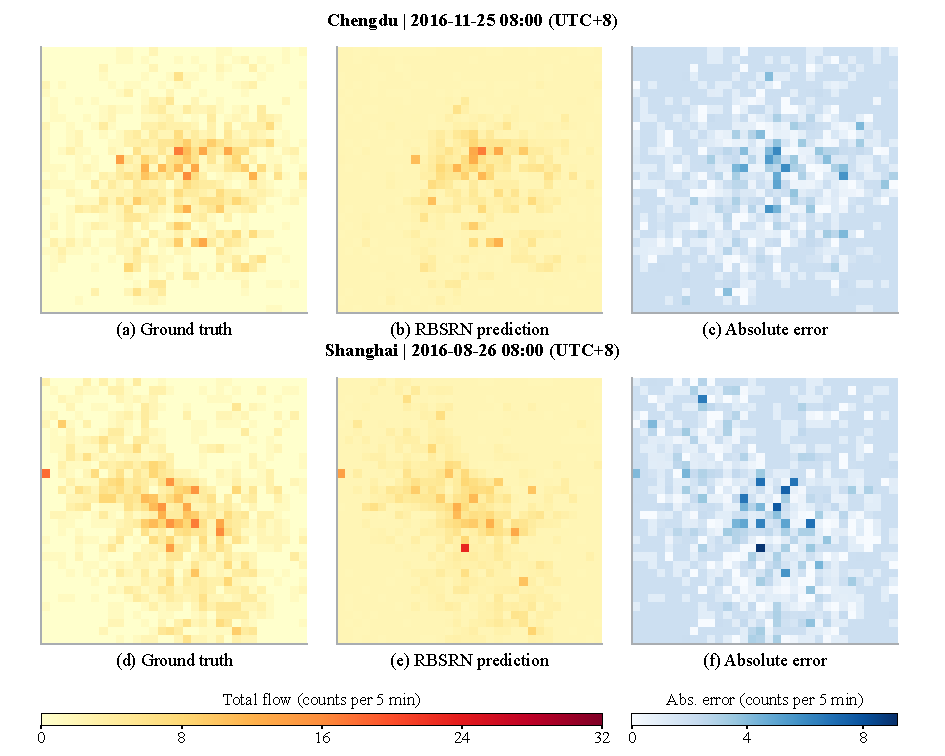
\includegraphics[width=\linewidth]{figures/spatial-fixed-morning.pdf}
  \caption{Example spatial predictions of total flow at H6 (08:00). The top and bottom rows show Chengdu and Shanghai, respectively. The columns show observations, predictions, and absolute errors.}
  \label{fig:rbsrn-spatial-h6}
\end{figure}
\FloatBarrier

% Scenario performance and analyses of the two residual pathways are included in 5.2.
% !TeX root = ../main.tex
% !TeX encoding = UTF-8

\subsubsection{Prediction Performance across Levels of Deviation from Routine Patterns}\label{sec:scenario-performance}\label{sec:exp-scenarios}

All-grid spatial statistics describe flow distribution at a given time. To examine prediction error under deviations from routine levels, we grouped observations by window, grid cell, and channel. At positions with positive H6 target flow, RBSRN was compared with 16 baselines. Chengdu scenario analysis and the subsequent residual diagnostics use a dedicated diagnostic checkpoint, whose full-test-set H6 MAE is 0.709952 for inflow and 0.709944 for outflow. The main Chengdu tables use the comparison checkpoint. Shanghai scenario analysis and residual diagnostics use the epoch-115 checkpoint reported in the main tables.

The routine-flow reference is the median training flow for the same grid cell, channel, 5-minute slot, and weekday/weekend type. We used deduplicated training-history timestamps that passed the quality checks. If a slot had fewer than four observations for one day type, the two types were pooled; if it had none, we used the grid-cell and channel median. We divided each observation's difference from its reference by a robust scale to obtain the standardized residual \(r_k\). The scale is the training residual median absolute deviation multiplied by 1.4826, with a lower bound of 1 count. The input-window deviation score is \(D=\frac{1}{12}\sum_{k=1}^{12}|r_k|\). For each city and channel, we pooled grid cells from training windows whose 12 historical steps passed the quality checks. The 50th, 80th, and 95th percentiles of \(D\) define four groups (Table~\ref{tab:scenario-group-thresholds}); boundary values enter the lower group.

% !TeX root = ../main.tex
\begin{table}[!htbp]
  \centering\footnotesize
  \caption{Scenario-group thresholds from training data}
  \label{tab:scenario-group-thresholds}
  \setlength{\tabcolsep}{4pt}
  \begin{tabular}{llrrrrrr}
    \toprule
    City & Channel & \(D_{50}\) & \(D_{80}\) & \(D_{95}\) & \(U_{75}\) & \(B_{1/3}\) & \(B_{2/3}\) \\
    \midrule
    Chengdu & Inflow & 0.166667 & 0.583333 & 1.083333 & 1.636364 & 0.279326 & 0.453125 \\
    Chengdu & Outflow & 0.166667 & 0.625000 & 1.083333 & 1.636364 & 0.287192 & 0.471179 \\
    Shanghai & Inflow & 0.281038 & 0.708333 & 1.096048 & 1.636364 & 0.311065 & 0.489387 \\
    Shanghai & Outflow & 0.250000 & 0.674491 & 1.083333 & 1.590909 & 0.311294 & 0.492517 \\
    \bottomrule
  \end{tabular}
\end{table}


\begin{figure}[!htbp]
  \centering
  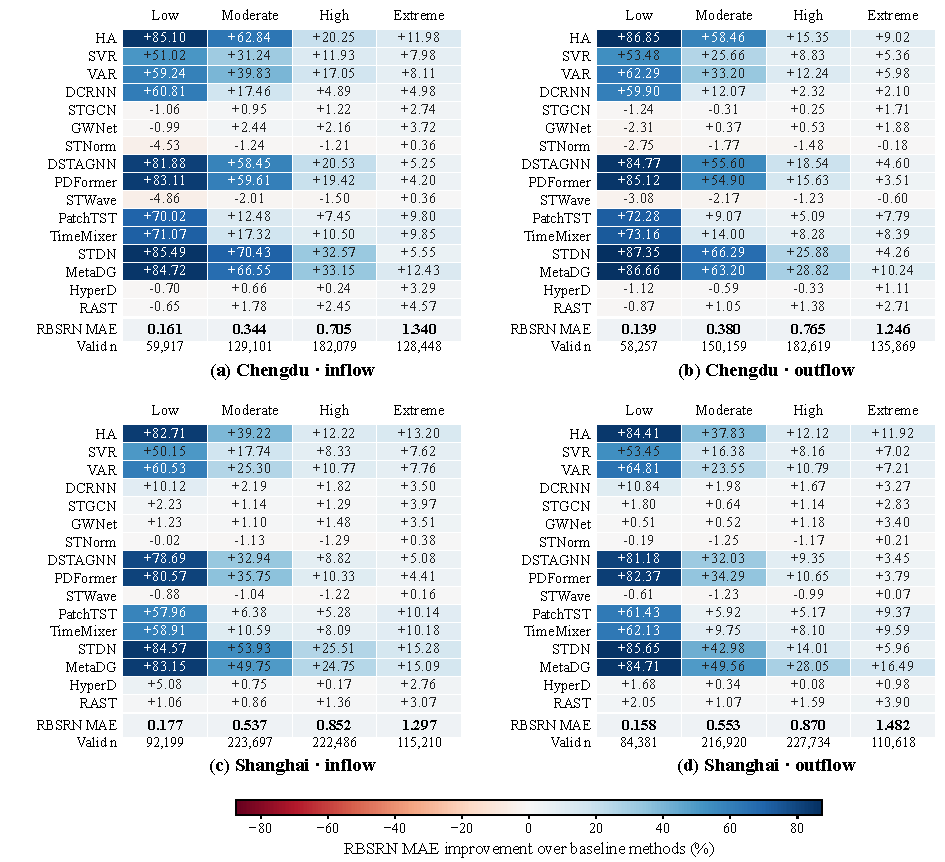
\includegraphics[width=\linewidth]{figures/scenarios/performance_h6_paper.pdf}
  \caption{RBSRN relative MAE at H6 across deviation groups.}
  \label{fig:scenario-performance}
\end{figure}

Figure~\ref{fig:scenario-performance} compares methods within each group; positive values indicate an MAE reduction relative to the corresponding baseline. In the Extreme group, RBSRN had the lowest MAE for Chengdu inflow, Shanghai inflow, and Shanghai outflow, with reductions of 0.36\%, 0.16\%, and 0.07\% relative to STWave. For Chengdu outflow, RBSRN ranked third, with MAE 0.60\% above STWave. STWave and STNorm had lower errors than RBSRN in the Moderate and High groups on all four tasks.

Absolute MAE increased with deviation level on all four tasks. Extreme-group MAE was 7.33--9.37 times the Low-group value. For Chengdu inflow, MAE increased from 0.161 to 1.340 while mean positive-target flow increased from 1.160 to 3.637 counts per 5 min, so the group differences reflect both deviation level and flow magnitude.

\subsubsection{Effects of SERR Residual Corrections across Recent-Change Scenarios}\label{sec:scenario-serr}

Within the high-deviation subset combining High and Extreme observations (\(D>D_{80}\)), recent-change intensity is defined by successive differences in historical standardized residuals:
\begin{equation}
  U=\frac{1}{11}\sum_{k=2}^{12}|r_k-r_{k-1}|.
  \label{eq:scenario-recent-change}
\end{equation}
The 75th percentile of \(U\) among high-deviation training samples separates Slow and Rapid groups; values above the threshold enter Rapid.

We examined each residual correction with a fixed-model residual-removal diagnostic. Model parameters, gates, and all other outputs were held fixed while one specified correction was subtracted from the final prediction:
\begin{equation}
  \Delta\mathrm{MAE}_{e}
  =\mathrm{MAE}(\widehat Y-C_e)-\mathrm{MAE}(\widehat Y),
  \label{eq:scenario-residual-removal}
\end{equation}
Here, \(C_e\) is the signed correction added to the prediction, including the original gating weight, learnable strength coefficient, and inverse-standardization scale. Removing the SERR self-evolution expert subtracts its weighted difference from the base prediction; removing the directed time-lagged expert subtracts its weighted correction; removing BCMS subtracts the full cross-region correction. Gating weights retain their original values and are not renormalized. A positive difference means that the correction reduced group-average MAE. Because the loss is nonlinear, differences for separate corrections are not additive. This diagnostic complements the independently retrained ablations in Section~\ref{sec:exp-ablation}: it measures sensitivity of one fixed model, whereas the ablations compare retrained configurations.

In Figure~\ref{fig:scenario-serr}, all 16 removal differences across the eight city--channel--change groups were positive. The self-evolution correction benefit in Rapid was 1.15--2.82 times the Slow-group benefit, whereas the directed time-lagged correction was smaller. Its Rapid-group benefit was higher than its Slow-group benefit in Chengdu and lower in Shanghai.

\begin{figure}[!htbp]
  \centering
  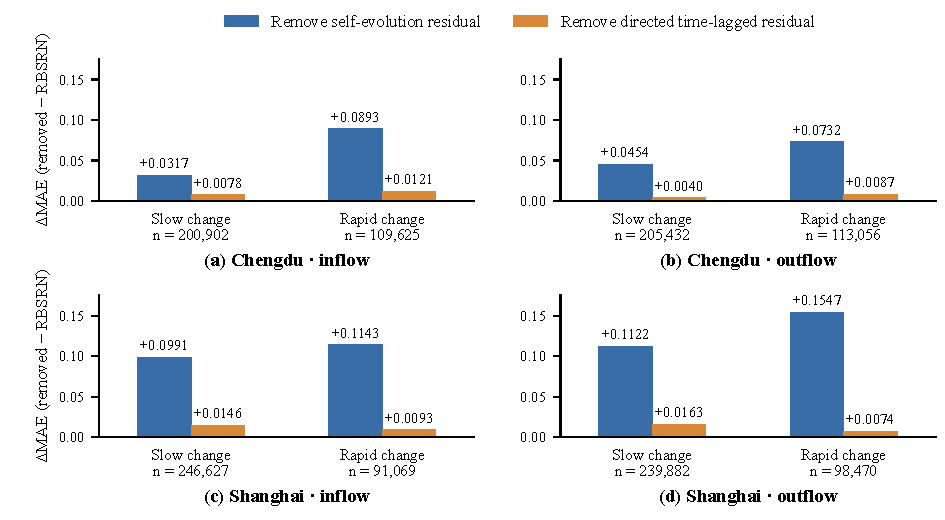
\includegraphics[width=0.92\linewidth]{figures/scenarios/serr_sensitivity_h6_paper.pdf}
\caption{H6 SERR residual-removal sensitivity by recent-change group.}
  \label{fig:scenario-serr}
\end{figure}

\subsubsection{Effects of BCMS Residual Corrections across Background Discrepancies and Forecast Horizons}\label{sec:scenario-bcms}

We measured source--target background similarity with a history-derived discrepancy proxy. Let \(\mathcal C_i\) denote the valid fixed candidate-source set for target cell \(i\), and let \(\bar r_i\) be its mean standardized residual over the 12 historical steps. For each channel, define
\begin{equation}
  B_i=\frac{1}{|\mathcal C_i|}\sum_{j\in\mathcal C_i}|\bar r_i-\bar r_j|.
  \label{eq:scenario-background-difference}
\end{equation}
The candidate set follows the model's fixed support. \(B_i\) describes discrepancy in the observed history and is separate from the low-frequency representation learned by BCMS. Tertile thresholds estimated from high-deviation training samples define Low, Medium, and High discrepancy groups (Table~\ref{tab:scenario-group-thresholds}). We removed the full BCMS correction at H1--H12 using Eq.~\eqref{eq:scenario-residual-removal}. Both figures report MAE changes in \(10^{-3}\) counts per 5 min; each cell is \(1000\times\Delta\mathrm{MAE}\).

Figure~\ref{fig:scenario-bcms} shows a consistent ordering across city, channel, and horizon: the mean benefit was largest in the Low group, followed by Medium and High. Of 144 background-group--horizon cells, 143 were positive; the only negative value was approximately \(-4.8\times10^{-6}\) for Chengdu outflow in the High group at H5. Benefits varied across horizons without a monotonic trend.

\begin{figure}[!htbp]
  \centering
  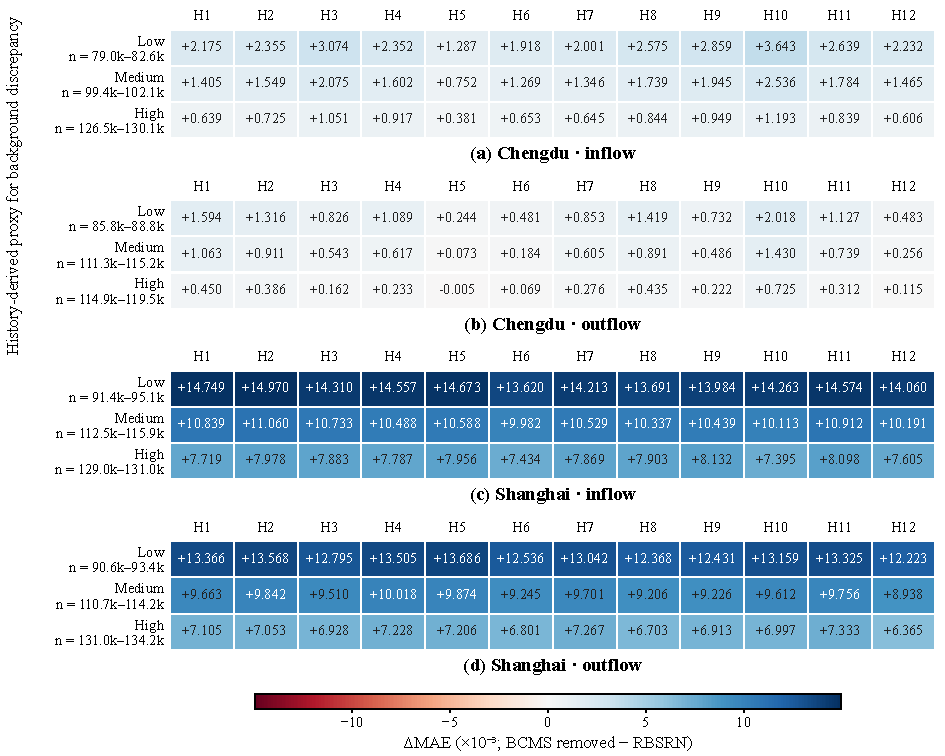
\includegraphics[width=0.92\linewidth]{figures/scenarios/bcms_sensitivity_horizons_paper.pdf}
\caption{BCMS residual-removal sensitivity in high-deviation scenarios.}
  \label{fig:scenario-bcms}
\end{figure}

Figure~\ref{fig:scenario-bcms-all} extends the analysis to the full test set with the same thresholds fitted from high-deviation training histories. All 144 removal differences were positive and exceeded the corresponding high-deviation values. The Low--Medium--High ordering persisted. For Shanghai inflow at H6, full-test differences were 0.025547, 0.015634, and 0.009873, compared with 0.013620, 0.009982, and 0.007434 in the high-deviation subset. The full-test analysis therefore shows that the average BCMS benefit extends beyond high-deviation samples.

\begin{figure}[!htbp]
  \centering
  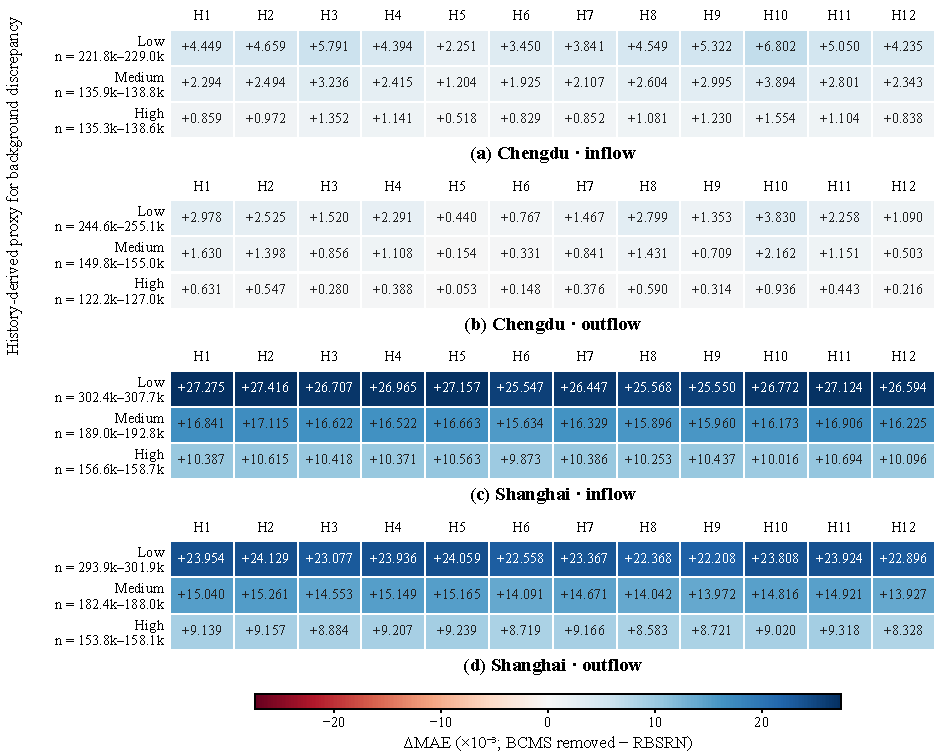
\includegraphics[width=0.92\linewidth]{figures/scenarios/bcms_sensitivity_horizons_all_test_paper.pdf}
\caption{BCMS residual-removal sensitivity across the full test set.}
  \label{fig:scenario-bcms-all}
\end{figure}



% !TeX root = ../main.tex
% !TeX encoding = UTF-8
\subsection{Ablation Study}\label{sec:exp-ablation}

We evaluated the three residual pathways with Chengdu ablations. A1 removes the self-evolution expert, A2 removes the directed time-lagged expert, and A3 removes BCMS. Each variant was retrained for up to 200 epochs with an early-stopping patience of 20 epochs. In A1 and A2, the remaining expert weights were renormalized after setting the removed weight to zero. Testing used the positive-target mask and AVG12 aggregation defined in Section~\ref{sec:exp-baselines-metrics}. Joint MAE and RMSE are the equal-weight averages of the inflow and outflow AVG12 values.

% !TeX root = ../main.tex
\begin{table}[!htbp]
  \centering
  \caption{Chengdu ablation results (AVG12)}
  \label{tab:serr-expert-ablation}
  \begingroup
  \linespread{1}\fontsize{9}{11}\selectfont
  \setlength{\tabcolsep}{3pt}
  \renewcommand{\arraystretch}{1.08}
  \begin{tabular*}{\linewidth}{@{\extracolsep{\fill}}lrrrrrr@{}}
    \toprule
    Model configuration & \shortstack{Inflow\\MAE} & \shortstack{Inflow\\RMSE} & \shortstack{Outflow\\MAE} & \shortstack{Outflow\\RMSE} & \shortstack{Joint\\MAE} & \shortstack{Joint\\RMSE} \\
    \midrule
    RBSRN & \ablationpolished{\textbf{0.7084}} & \ablationpolished{\textbf{1.2935}} & \ablationpolished{\textbf{0.7087}} & \ablationpolished{\textbf{1.2235}} & \ablationpolished{\textbf{0.7085}} & \ablationpolished{\textbf{1.2585}} \\
    w/o Self-evolution expert (A1) & \ablationpolished{0.7129} & \ablationpolished{1.3037} & \ablationpolished{0.7121} & \ablationpolished{1.2270} & \ablationpolished{0.7125} & \ablationpolished{1.2653} \\
    w/o Directed time-lagged expert (A2) & \ablationpolished{0.7105} & \ablationpolished{1.3048} & \ablationpolished{0.7099} & \ablationpolished{1.2264} & \ablationpolished{0.7102} & \ablationpolished{1.2656} \\
    w/o BCMS (A3) & \ablationpolished{0.7109} & \ablationpolished{1.3014} & \ablationpolished{0.7102} & \ablationpolished{1.2276} & \ablationpolished{0.7105} & \ablationpolished{1.2645} \\
    \bottomrule
  \end{tabular*}
  \endgroup
\end{table}

\FloatBarrier

Table~\ref{tab:serr-expert-ablation} shows that the full RBSRN had the lowest error on all six metrics. Removing any branch increased MAE and RMSE for both flows. Removing the self-evolution expert increased joint MAE by 0.56\%, the largest increase among the variants. Removing the directed time-lagged expert increased joint RMSE by 0.56\%, compared with 0.54\% for removing self-evolution. The two experts therefore contribute through different error measures, with self-evolution having the larger effect on joint MAE.

Removing BCMS increased joint MAE and RMSE by 0.28\% and 0.48\%, respectively, with higher errors for both flows. The full model performed best when self-evolution, directed time-lagged association, and background-conditioned message selection were combined.
\FloatBarrier


% !TeX root = ../main.tex
% !TeX encoding = UTF-8
% !TeX spellcheck = none
\subsection{Hyperparameter Sensitivity Analysis}\label{sec:exp-hyperparameters}

\hpupdated{We conducted one-factor-at-a-time validation experiments on Chengdu to examine how SERR gating capacity, BCMS representation capacity, and the initial values of two residual pathways affect prediction error. The SERR gating hidden dimension and the BCMS internal representation dimension each took values in \(\{8,16,32,64,128\}\). Both \(\alpha_0\) and \(\beta_0\) took values in \(\{0,0.001,0.01,0.05,0.1\}\). They specify the initial values of the learnable residual parameters defined in Sections~\ref{sec:serr} and~\ref{sec:bcms}, respectively, and these parameters continue to update during training. The reference configuration was \((32,32,0,0)\), as used in the main comparison experiments. We changed one parameter at a time while keeping all other settings fixed. \editorialupdated{Bold tick labels indicate the reference configuration, and the minimum within each group was determined from unrounded results.} Training, checkpoint selection, and validation aggregation followed Sections~\ref{sec:exp-implementation} and~\ref{sec:exp-datasets}.}

\hpupdated{We first constructed the model with the reference configuration and replaced the gating or BCMS module only when its dimension differed from 32. Residual initial values were assigned directly to the learnable parameters. Neither training nor validation used additional splitting into microbatches.}

\hpupdated{All four parameters produced only small changes in joint validation error within the tested ranges (Figure~\ref{fig:hyperparameter-joint}). We calculated each group's relative range as the difference between its maximum and minimum errors divided by the error of the reference configuration. Across the four groups, this range was below 0.15\% for joint MAE and below 0.35\% for joint RMSE.}

\begin{figure}[!htbp]
  \centering
  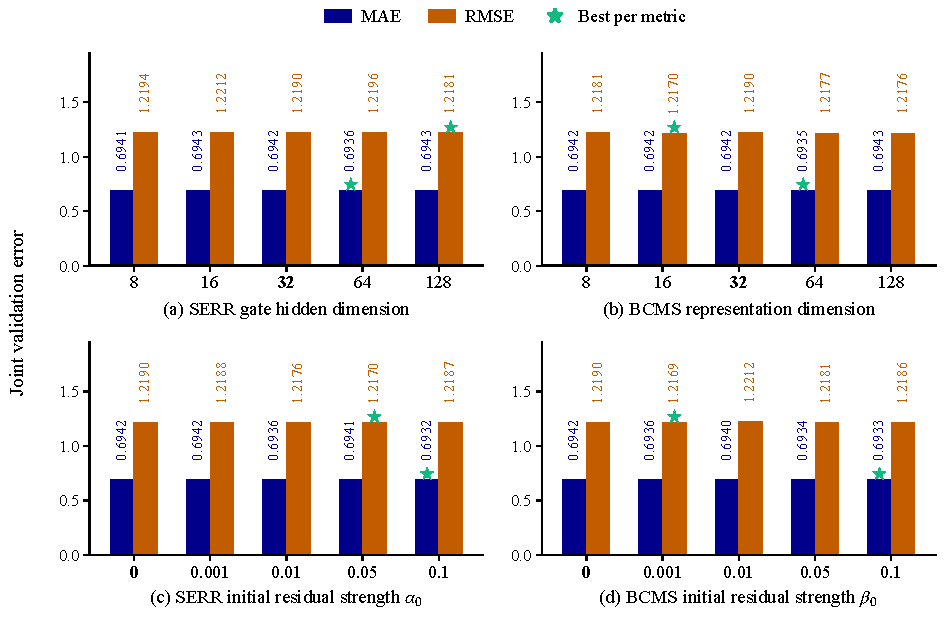
\includegraphics[width=\linewidth]{figures/hyperparameter-joint.pdf}
  \caption{\editorialupdated{Hyperparameter sensitivity of joint validation metrics on the Chengdu dataset.}}
  \label{fig:hyperparameter-joint}
\end{figure}

\hpupdated{Increasing the hidden dimension did not consistently reduce error, and the lowest joint MAE and RMSE occurred at different dimensions. The best positive initial values of the residual parameters provided only small improvements over zero initialization. The two metrics likewise did not share a single optimal initial value.}

\hpupdated{Figure~\ref{fig:hyperparameter-flow} presents the complete results for each flow channel. The small changes in joint error also included different responses across channels. For the SERR gating dimension, inflow MAE was lowest at 64, whereas outflow MAE was lowest at 8. Thus, the two flow channels responded differently to gating capacity.}

\begin{figure}[!htbp]
  \centering
  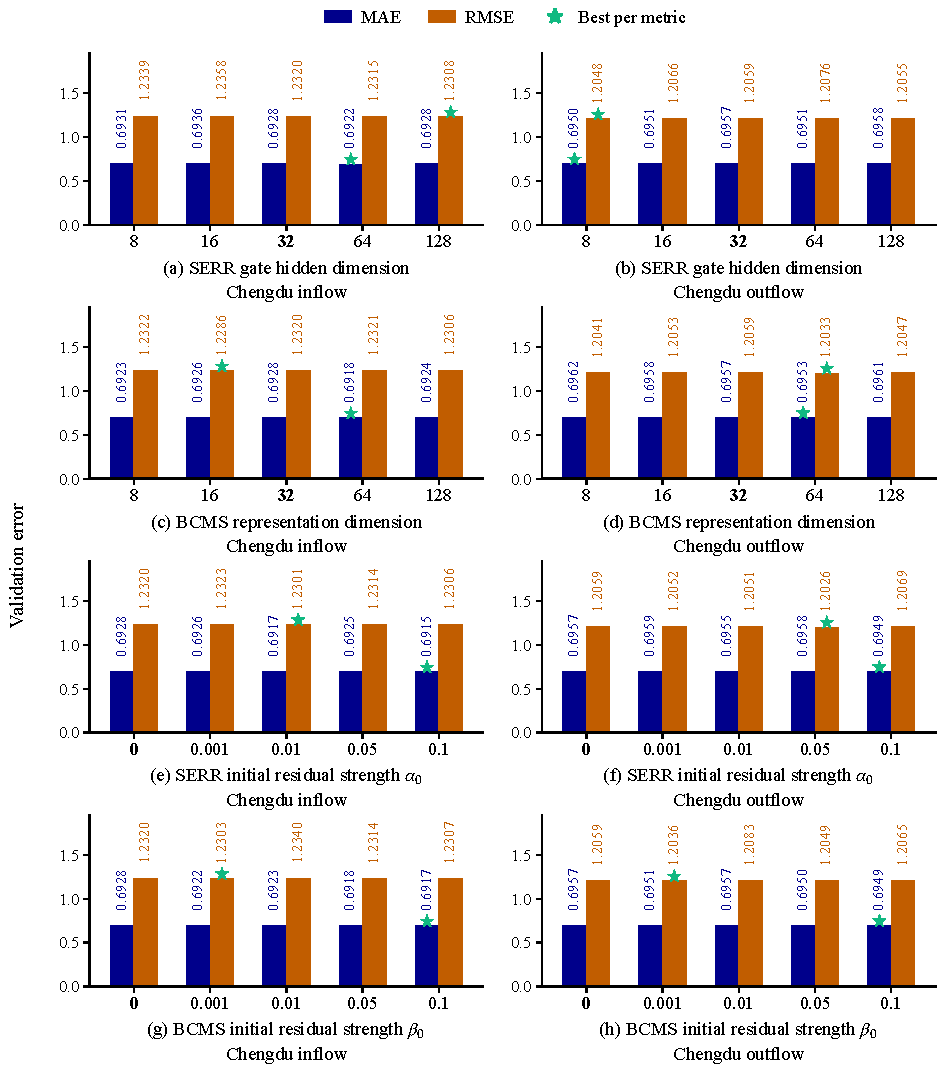
\includegraphics[width=\linewidth]{figures/hyperparameter-flow.pdf}
  \caption{\editorialupdated{Hyperparameter sensitivity for inflow and outflow on the Chengdu dataset.}}
  \label{fig:hyperparameter-flow}
\end{figure}
\FloatBarrier


% !TeX root = ../main.tex
\subsection{Model Size and Inference Efficiency}\label{sec:exp-efficiency}

With both the gating and BCMS dimensions set to 32, RBSRN contains approximately 7.071 million trainable parameters. We evaluated inference efficiency using the Chengdu checkpoint from the main comparison experiments. Each batch-size setting used a single NVIDIA A100-SXM4-40GB GPU with FP32 tensors; the remaining computing environment is described in Section~\ref{sec:exp-implementation}. Each window supplies 12 historical flow steps and jointly produces inflow and outflow forecasts for 1,024 nodes over the next 12 steps.

For batch size 1, we used compiled BCMS operators and CUDA Graph, with 20 warm-up iterations followed by 100 timed iterations. For batch size 64, we used compiled BCMS operators, with 10 warm-up iterations followed by 30 timed iterations. CUDA synchronization was performed before and after each measurement. We report the median and 95th percentile (P95), which describe typical execution time and tail latency within these measurements, respectively.

Forward-only timing includes model computation on GPU-resident inputs and excludes copying new inputs. End-to-end timing covers memory-resident data access, wavelet decomposition, normalization, state-evidence construction, CPU/GPU transfers, model inference, inverse standardization, and returning results to the CPU. It also includes input updates before CUDA Graph replay. Both measurements exclude startup preparation, offline graph construction, and cold disk reads. Startup preparation comprises initialization, compilation, graph capture, and warm-up.

\begin{table}[!htbp]
	\centering
	\small
	\caption{RBSRN inference time on the Chengdu dataset}
	\label{tab:inference-latency}
	\begin{tabular*}{\linewidth}{@{\extracolsep{\fill}}lcrrrr@{}}
		\toprule
		Inference setting & Batch size
		& \multicolumn{2}{c}{\shortstack{Forward only\\ms/batch}}
		& \multicolumn{2}{c}{\shortstack{End to end\\ms/batch}} \\
		\cmidrule(lr){3-4}\cmidrule(lr){5-6}
		& & Median & P95 & Median & P95 \\
		\midrule
		\shortstack[l]{Single-window\\forecasting} & 1  & 15.907   & 15.930   & 19.228   & 19.507 \\
		Batch forecasting   & 64 & 1138.819 & 1310.517 & 1280.394 & 1464.308 \\
		\bottomrule
	\end{tabular*}
\end{table}

Table~\ref{tab:inference-latency} reports median forward-only and end-to-end latencies of 15.907\,ms and 19.228\,ms for single-window forecasting, with an end-to-end P95 of 19.507\,ms. In this test environment, the measured computation time fit within a 5-minute update cycle. At batch size 64, the median end-to-end time was 1,280.394\,ms/batch, and the amortized forward-only time was 17.794\,ms/window. The batch-size-1 measurements characterize the response time of an individual request.

The inference configurations above used the same model checkpoint. We compared each against the reference implementation at the same batch size. At batch size 64, checking all 1,723 test windows yielded a maximum absolute prediction difference of \(7.63\times10^{-6}\). Batch size 1 passed a sampled check against the reference at the same batch size. Aggregate forecasting metrics were similar across the two batch sizes, although individual predictions were not identical. All main accuracy results were evaluated at batch size 64.

\FloatBarrier

